\pagebreak
\section{Finite case of CTA}

\subsection{Context depended operations}

Following earlier definitions one can proceed with some basic transformations of binary strings. Consider a boolean logic operation like $xor$ computed over values of two strings $\{x_n, y_n\} \subset B_n, n \in \nat$ individually. The result of such string operation $z_n$ can be obtained as value-wise or element-wise addition modulo 2, s.t. $z_n(j) = x_n(j) \oplus y_n(j), \forall j \in J $, where $J$ is an enumeration or index set. 

Computing a sequence $z_n(j), \forall j \in J$ is done index by index, defined by the shared enumeration set $J$ with each position being treated independently. Meaning that the end result does not depend on the order of operations as long as the bits of the outcome binary string $z_n$ can be put together in the right order $\forall j \in J$. We will call such operations \textit{context-free operations}. 

A different situation is a special case when some basic binary operation is applied to strings of bits in strictly dependent order. Indeed, the trivial case of performing a $xor$ operation over two binary strings can be computed in parallel and the outcome will be always the same over and over again as long as we can match the indexes. 

However, if one can control how the resulting $z_n$ string is produced by adding some memory property to store previously computed or observed states, one will most likely come up with a stateful process of a binary string transformation. We will refer to such string operations augmented with the memory state as \textit{context depended operations}.

\begin{definition}\label{def_cursor}
  Consider an input binary string $b_n, n \in \nat$ and a cursor $b_n(k)$ pointing at some index $0 \leq k < n$. A context of a fixed length $m < n$ observed to the left of $k$ is a \textit{prefix} enumerating values before index $k$ as $\bos b_n(k-m),..,b_n(k-1)\eos.$
\end{definition}

\subsection{Context Transformation Algorithm}

Let us illustrate how one of such context depended algorithms can work. Let $b_n$ be a finite input string. We will use a state lookup table (see fig. \ref{fig:cta}) for state tracking purposes. One needs to choose the length of the context as $m < n, m \in \nat$, so that the left-hand of the lookup table will consists of all possible context strings of such length $C_m = \{\bos 000..00\eos_m, \bos 000..01\eos_m, .. \\ \bos 111..11\eos_m\},\, |C_m| = 2^m$ that can be potentially found while traversing $b_n$ with $k \in J = \bos 0,\,..,\,n-1\eos$. 

\begin{figure}[h!]
  \centering
  \begin{subfigure}[b]{0.9\linewidth}
    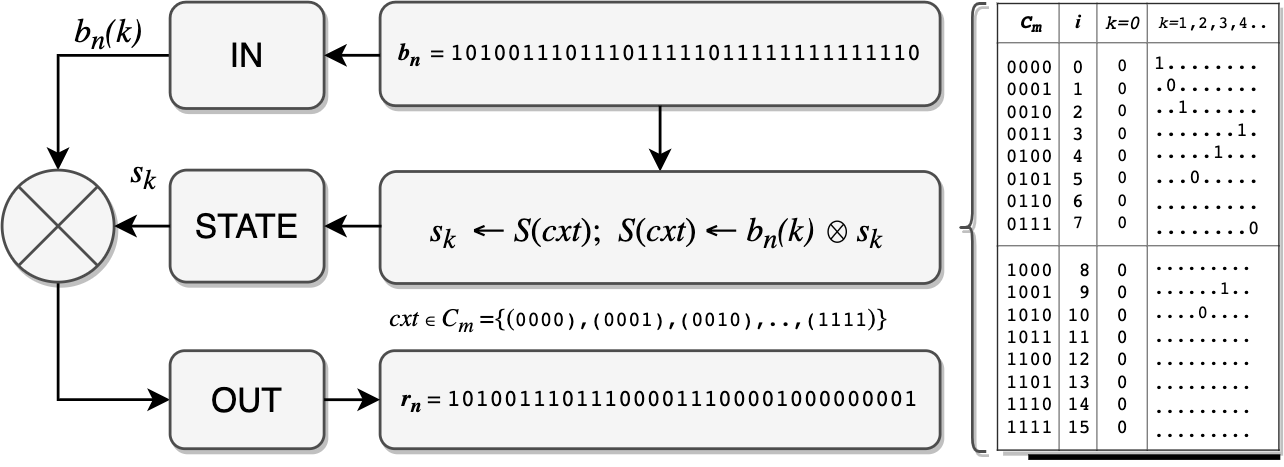
\includegraphics[width=\linewidth]{appendix/CTA.png}
  \end{subfigure}
  \caption{Context transformation algorithm. Finite case.}
  \label{fig:cta}
\end{figure}

For convenience, prefix values which have not yet been observed before some cursor $k < m$ are padded with zeros. For example, for $k \geq 0$ and $m=4$ first few observed context strings will be padded until no more padding is required as in $(0000, 000x, 00xx, 0xxx, xxxx)$, where $x \in \{0,1\}$ is a value placeholder and $k \geq m$. Alternatively one can imaging a sliding window of fixed length $m < n$ moving from left to right over the indexes of $b_n$ to observe all found context strings of that length.

We define a finite case of \textit{CTA} as following: 

\begin{enumerate}
\item \textbf{take} a finite binary string $b_n$ as input - for example,\\ let $b_n = \bos101001110111011111011111111111110\eos_{n=33}$
\item \textbf{choose} the size of the context as $m < n, m \in \nat$ - for example, $m=4$
\item \textbf{point} cursor at position $k=0,k \in J$, so that we can access first value $1 \leftarrow b_n(k)$ at the beginning of $b_n$
\item \textbf{initialize} all unobserved states in the state table with zeros \\$S(cxt) \leftarrow 0, \forall cxt \in C_m$ 
\item \textbf{set} the observed context $cxt \leftarrow \bos 000..00\eos_m$
\item \textbf{shift} bits of the observed context to the left by dropping a value at the first index $cxt(0)$ 
\item \textbf{update} the observed context string by appending the input value at cursor $cxt \leftarrow \bos cxt(1), cxt(2), .., cxt(m-1), b_n(k)\eos_m$
\item \textbf{take} $s_k \leftarrow S(cxt)$
\item \textbf{output} next bit $r_n(k) \leftarrow b_n(k) \oplus s_k$
\item \textbf{update} memory state for observed context $S(cxt) \leftarrow b_n(k) \oplus s_k$, which will be $1$ if the state has changed and $0$ otherwise
\item \textbf{if} $k = n$ and cursor points at the end of the input string, 
\\ \textbf{then} transformation is complete and we can terminate the algorithm
\\ \textbf{else} move cursor to the next index $ k \leftarrow k + 1$ at the input string $b_n$ (from left to right) and continue by jumping back to step (6) 
\end{enumerate}

\subsection{Bijectivity of CTA}

Above we have defined the CTA as a context-depended algorithm that takes a finite binary string $b_n$ as an input and uses a simple $xor$ operation applied to the input bits and the memory states to produce an output string $r_n$. For example and as shown on fig. \ref{fig:cta} - $r_n \leftarrow CTA(b_n)$, so for the sample input the CTA result is: \begin{align*}
b_n = \bos101001110111011111011111111111110\eos
\\ r_n = \bos101001110111000011100001000000001\eos
\end{align*}

Interestingly enough, $xor$ operation on binary strings can be easily reversed. Which means, that one can also define an inverse version of the algorithm such that it will take $r_n$ as input and produce the original values of $b_n$ as output - $b_n \leftarrow {CTA}^{-1}(r_n)$.

\begin{theorem}If a context transformation algorithm on finite binary strings $B_n$ can be represented by a function ${CTA}_{m}: B_n \to B_n$, where context length is $m < n: m,n \in \nat$, then ${CTA}_{m}$ is both a total computable and bijective function.\end{theorem}
\begin{proof}There exists a direct and inverse implementation of ${CTA}_{m}$ in Turing-complete programming language\footnote{See "CTA - code listing" in appendix - for direct and inverse algorithm implementation in python}.\end{proof}

